% Penjelasan dasar cosine (1) dan contoh 2D (2), teks seminimal mungkin.
% Kompilasi (dari folder ini): pdflatex cosine_dasar.tex && pdftoppm -png -r 300 -singlefile cosine_dasar.pdf cosine_dasar
\documentclass[border=6pt]{standalone}
\usepackage{amssymb}
\usepackage{mathptmx}
\usepackage{tikz}
\usetikzlibrary{arrows.meta, calc}

\definecolor{ink}{HTML}{3A3936}
\definecolor{muted}{HTML}{8A8984}
\definecolor{modelE}{HTML}{2A78D6}
\definecolor{augE}{HTML}{EB6834}

\tikzset{
  every node/.style={font=\small, text=ink, align=center},
  title/.style={font=\normalsize\bfseries, anchor=west},
  vec/.style={-{Stealth[length=3mm]}, line width=1.8pt},
  proj/.style={dashed, line width=0.9pt, draw=muted},
}

\begin{document}
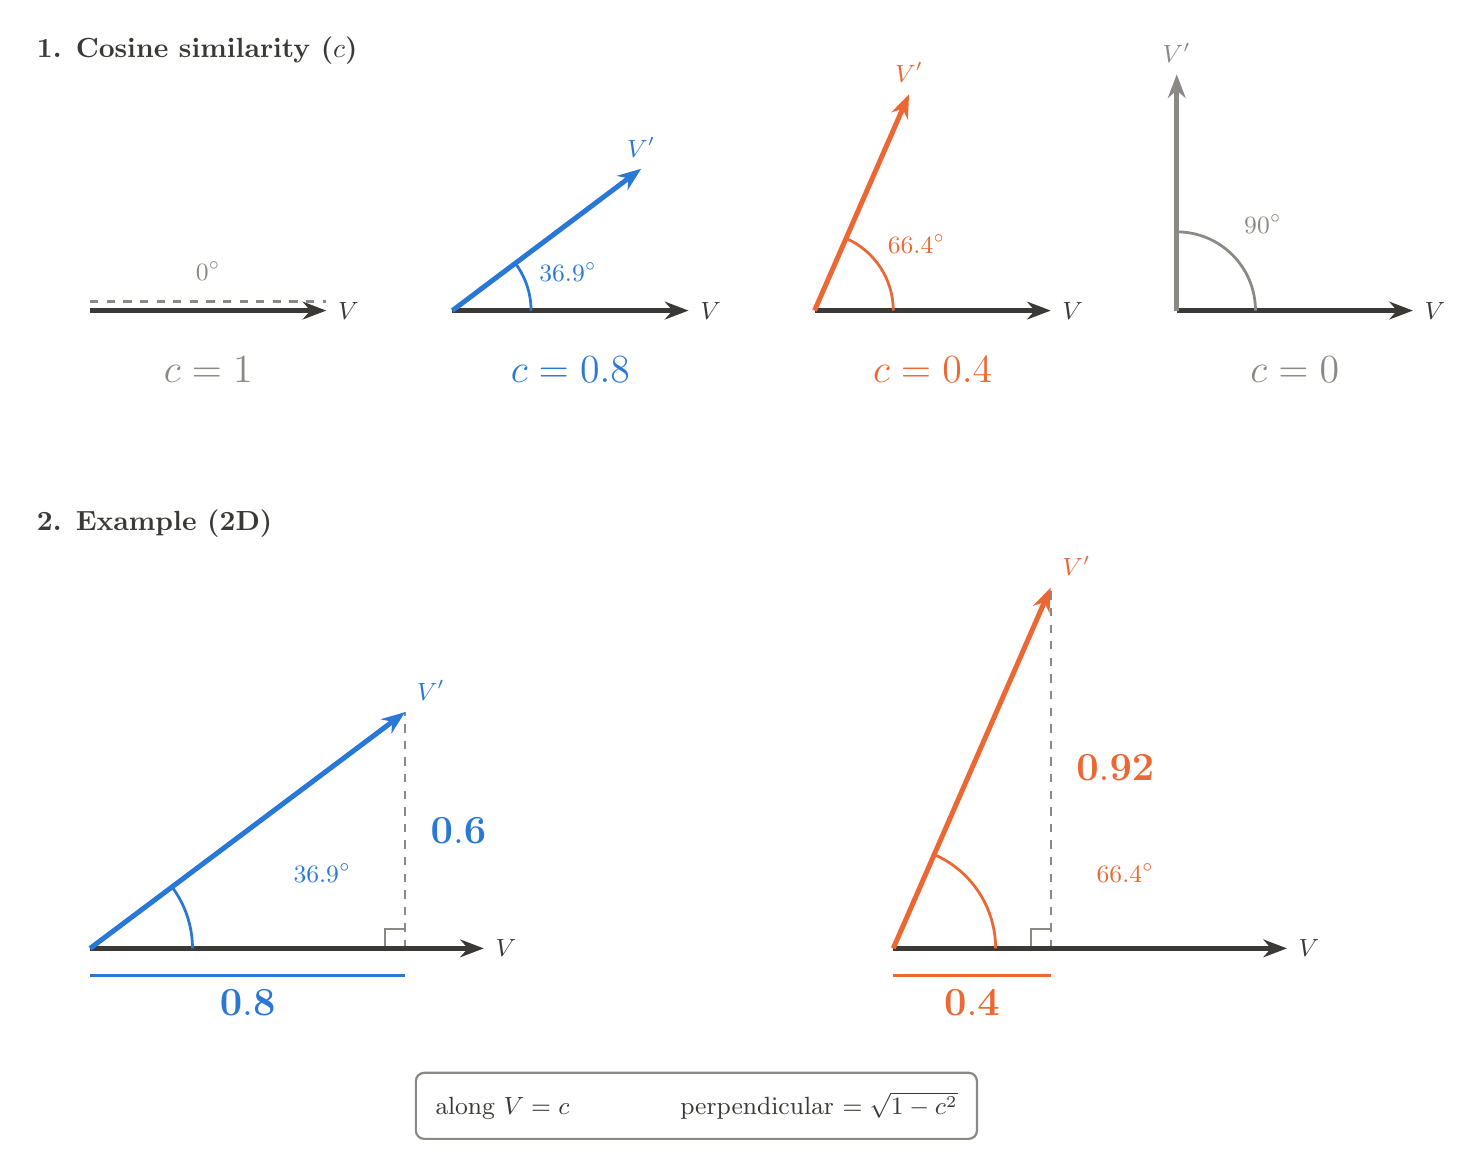
\begin{tikzpicture}

% ================= 1. cosine =================
\node[title] at (-0.8, 3.3) {1. Cosine similarity ($c$)};

\foreach \x/\ang/\col/\cval in {0/0/muted/1, 4.6/36.9/modelE/0.8, 9.2/66.4/augE/0.4, 13.8/90/muted/0} {
  \draw[vec, ink] (\x,0) -- (\x+3.0,0) node[right] {$V$};
  \ifdim \ang pt>0pt
    \draw[vec, \col] (\x,0) -- ($(\x,0)+(\ang:3.0)$) node[above, text=\col] {$V'$};
    \draw[\col, line width=1pt] ($(\x,0)+(1.0,0)$) arc (0:\ang:1.0);
    \node[font=\small, text=\col] at ($(\x,0)+({\ang/2}:1.55)$) {$\ang^\circ$};
  \else
    \draw[muted, dashed, line width=1pt] (\x,0.12) -- (\x+3.0,0.12);
    \node[font=\small, text=muted] at (\x+1.5,0.5) {$0^\circ$};
  \fi
  \node[font=\Large, text=\col] at (\x+1.5,-0.75) {$c=\cval$};
}

% ================= 2. contoh 2D =================
\node[title] at (-0.8,-2.7) {2. Example (2D)};

\foreach \c/\sv/\s/\col/\xo/\lp in {0.8/0.6/0.6/modelE/0/18, 0.4/0.92/0.9165/augE/10.2/18} {
  \begin{scope}[shift={(\xo,-8.1)}]
    \pgfmathsetmacro{\a}{acos(\c)}
    \pgfmathsetmacro{\px}{\c*5}
    \pgfmathsetmacro{\py}{\s*5}
    \draw[proj] (\px,0) -- (\px,\py);
    \draw[muted, line width=0.7pt] (\px-0.25,0) -- (\px-0.25,0.25) -- (\px,0.25);
    \draw[vec, ink] (0,0) -- (5,0) node[right] {$V$};
    \draw[vec, \col] (0,0) -- (\px,\py) node[above right, text=\col] {$V'$};
    \draw[\col, line width=1pt] (1.3,0) arc (0:\a:1.3);
    \node[font=\small, text=\col, fill=white, inner sep=1pt] at ({\lp}:3.1) {$\pgfmathprintnumber[precision=1]{\a}^\circ$};
    \draw[\col, line width=1.1pt] (0,-0.35) -- (\px,-0.35);
    \node[text=\col, below] at (\px/2,-0.4) {\Large $\mathbf{\c}$};
    \node[text=\col, anchor=west] at (\px+0.2,\py/2) {\Large $\mathbf{\sv}$};
  \end{scope}
}

\node[draw=muted, rounded corners=3pt, line width=0.8pt, fill=white, inner sep=7pt] at (7.7,-10.1)
  {along $V=c$ \qquad\qquad perpendicular $=\sqrt{1-c^{2}}$};

\end{tikzpicture}
\end{document}
